
\documentclass[journal,10pt,twocolumn]{article}
\usepackage{graphicx}
\usepackage[margin=0.5in]{geometry}
\usepackage{amsmath}
\usepackage{array}
\usepackage{booktabs}
\usepackage{amssymb}
\title{\textbf{Matrix Assignment}}
\author{lakshmi kamakshi}
\date{September 2022}

\begin{document}

\maketitle
\paragraph{\textit{Problem Statement} -Two concentric circles are of radii 5cm and 3cm. Find the length of the chord of the larger circle which touches the smaller circle.}
\vspace{5mm}

\section*{Solution}

Given the radii of the circles : $3cm$,$5cm$

 p = $5cm$ , a = $3cm$.
Let,
\begin{eqnarray}
	\boldsymbol{O}-\boldsymbol{A} = \boldsymbol{p}
\\	\boldsymbol{O}-\boldsymbol{P} = \boldsymbol{a}
\\	\boldsymbol{P}-\boldsymbol{A} = \boldsymbol{o}
\end{eqnarray}
\\ From the triangle law of addition of vectors:
\begin{eqnarray}
 \boldsymbol{p} = \boldsymbol{a} + \boldsymbol{o}
\\ \boldsymbol{o} = \boldsymbol{p} - \boldsymbol{a}
\end{eqnarray}
\\ find the magnitude of the vector o 
	\begin{eqnarray}
		||\textbf{o}||^2 = ||\textbf{p-a}||^2
		\\	||\textbf{o}||^2 = |\textbf{p-a}||\textbf{p-a}|^T
		\\||\textbf{o}||^2 = ||\textbf{p}||^2+||\textbf{a}||^2-2\textbf{p.a}^T
		\\ ||\boldsymbol{o}||^2 = \boldsymbol{25 + 9 -2(|\textbf{p}||\textbf{a}|)(cos\theta)}
\end{eqnarray}


\begin{figure}[h]
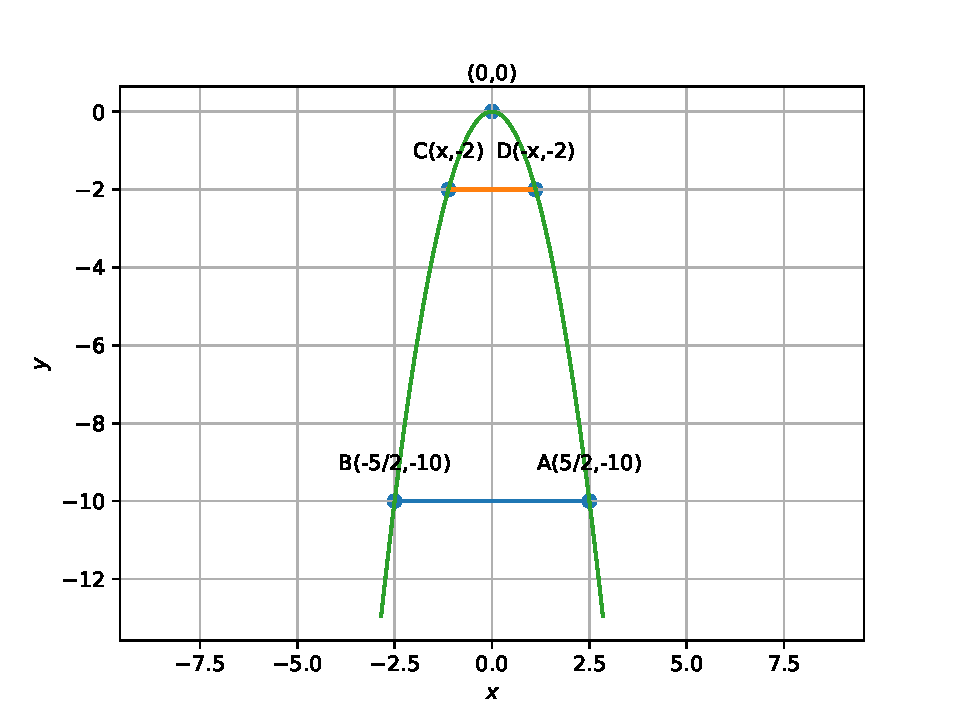
\includegraphics[width=1\columnwidth]{fig.pdf}
\end{figure}
 From the figure, in $\triangle$ OPA:
\begin{equation}
\boldsymbol{cos\theta} = \boldsymbol{\frac{3}{5}}
\end{equation}
\\ Substitute eqn10 value in eqn9
\begin{eqnarray}
||o||^2 = 34 - 2(3)(5)(\frac{3}{5})
\\ ||o||^2 = 34-18
\\ ||o||^2 = 16
\\ \boldsymbol{||o||} =\boldsymbol{4}
\end{eqnarray}
Similarly, in $\triangle$ OPB,
\begin{eqnarray}
	\boldsymbol{P}-\boldsymbol{B} = \boldsymbol{b}
\\	||\boldsymbol{b}|| = 4
\end{eqnarray}
\begin{eqnarray}
	||\boldsymbol{A-B}|| =|\boldsymbol{o}|+|\boldsymbol{b}|
	\\ \boldsymbol{A-B} = 4+4
	\\ \boldsymbol{A-B} = \boldsymbol{8}
\end{eqnarray}
\\ Therefore, the length of the required chord is $8cm$

\section*{Construction}
The input parameters are the lengths a and p.\\
\setlength \extrarowheight{2pt}
\centering
	\begin{tabular}{|c|c|c|}
	\hline
	\textbf{symbol}&\textbf{value}&\textbf{description}\\
	\hline
	a&3&OP\\
	\hline
	p&5&OA\\
	\hline
		$\theta$&acos($\frac{a}{p}$)&$\angle$O\\
	\hline
	A&$\sqrt{p^2-a^2}%
	\begin{pmatrix}
	cos\theta\\
	sin\theta\\
	\end{pmatrix}$%
	&Point A\\
	\hline
\end{tabular}
\end{document}
